\section{Introduction}
   
Maxwell's laws of electromagnetics indicate that light 
has wave-like properties,
in fact light has dual properties being wave-like and particle-like.  
In this class we will be studying the wave-like properties of light.  In 
Chapters~\ref{ch:optics} and \ref{ch:imaging}, 
we made the {\it ray approximation} which states that
a wave moves through a medium in a straight line.  If the wave
meets a barrier with an opening there are three possibilities that arise
depending on the width, $a$, of the opening.  First, for $a \gg \lambda$ 
where $\lambda $ is the wavelength of the wave of light,
the wave continues to travel in a
straight line (apart from some edge affects).  Second, for $a \sim \lambda$, 
the wave spreads out from the opening, the ray is 
{\bf diffracted}; last, for $a \ll \lambda$ the opening acts like a point 
source of waves.  The ray approximation is {\it invalid} for the second and 
third cases.
These three possibilities are depicted in Fig.~\ref{fig:diff:opening}.

\begin{figure}[htb]
\centering 
\epsfxsize=8cm 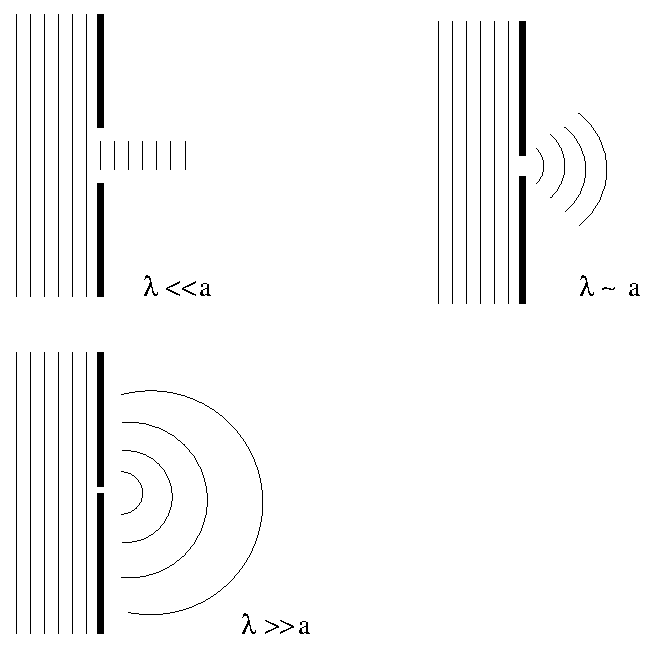
\includegraphics[scale=0.6]{10_diffraction/opening.eps}
\caption{The three possible scenarios for light's path  through an opening.
The top left figure depicts light ``unaffected'' by the opening, the
top right depicts diffraction effects, and the bottom depicts the opening 
as a point source of light.}
\label{fig:diff:opening}
\end{figure}

We are studying the wave-like properties of light as 
demonstrated by the phenomenon of diffraction, interference, and 
polarization (Chapter~\ref{ch:pol}).  For this lab, we will be using openings 
whose widths are of the order of the wavelength of light; therefore,
we will be dealing with waves spreading out in all directions.  The 
ray approximation we used in Chapters~\ref{ch:optics} and \ref{ch:imaging}
will {\bf no longer be 
valid}.   Since we are treating light like a wave, we will be able to 
apply the properties we have learned about waves, most importantly that 
they obey the superposition principle and thus interfere.  

The following theory section is divided into seven subsections. 
After a description of references,  
we will go through an introduction to diffraction and interference 
phenomenon.  Next we will study the two-slit interference pattern in detail,
ignoring diffraction effects in the limits where each slit behaves as a 
point source, followed by a less detailed multiple-slit 
interference subsection.  Then the diffraction grating is introduced.
The final two subsections reintroduce diffraction for the single slit and 
multiple slits, there we will study how diffraction determines the availability
of light for our study of interference.  

We will be performing four types of experiments.  First, you will
investigate the phenomenon of diffraction using a single slit.  Second,
you will use a slide with two slits to study two-slit interference and 
diffraction.  The same slide also has some multiple slits on it which
you will use to study multiple-slit interference and diffraction.  
Finally, you will use a diffraction grating to study the effects of
having 5000 lines (or slits) per cm.    
\\              
\section{Theory}

\subsection{References}

Serway addresses the interference of light waves in Chapter~37 
(Interference of Light Waves), and cursorily discusses diffraction
in Chapter~38 (Diffraction and Polarization). The single slit
diffraction pattern appears in Section~38.2, and the diffraction
grating shows up in Section~38.4. We will discuss these and other
effects here.

\subsection{Diffraction and Interference}

Light is an electromagnetic {\it wave}; therefore, just 
as two waves can add together destructively or constructively, so can
light.  In constructive interference,
the two wave amplitudes add together such that the resultant wave's amplitude
is greater than either individual's amplitude.  In destructive interference,
the amplitude of one wave ``cancels'' the amplitude of the other wave.  
In order to observe the interference of two waves, we need coherent,
monochromatic sources.  Coherent means the the sources have the same phase,
we will label the phase $\phi$.  Monochromatic means that the sources have
the same wavelength, $\lambda$.   Given these conditions, we will
use a laser as our light source since a laser is a source of 
monochromatic light,
and we will be illuminating a slide with slits in it thus creating 
sources of waves that are in phase at the slits.  

If light really did travel in straight line paths (like what we investigated 
in Chapters~\ref{ch:optics} and \ref{ch:imaging}) 
there would be no overlap, no interference pattern (see
the top left figure in Fig.~\ref{fig:diff:opening}).  
What really happens is that light, when incident upon an opening, 
deviates from 
a straight line path and enters the region that would otherwise be in 
shadow.  The divergence of light from
its initial path of travel is called diffraction. 
Diffraction generally occurs when light
passes through a small opening, around sharp corners, or past sharp edges.
We will be assuming {\bf very narrow slits}; therefore,
we will expect diffraction.

\subsection{Two-Slit Interference}

{\it For now only}, 
let's assume that the two slits are so narrow that they act as two wave 
sources, so $a \ll \lambda$, as in the bottom picture in 
Fig.~\ref{fig:diff:opening}.  With this set-up we can study the interference
of two waves and then add the effects of diffraction later.  We know
that waves interfere constructively and destructively from our previous
studies of waves in physics; therefore, we expect to see bright and
dark areas, respectively, on the viewing screen.

Consider the diagram in Fig.~\ref{fig:diff:2-slit}. 
It shows two openings of 
width $a$ whose centers are separated by a distance $d$. We want to calculate 
the intensity as a function of position on a screen a distance $L$ away. 
Consider point~P which makes an angle of $\theta$ with respect to the center 
normal. If we illuminate both slits from the left with a monochromatic wave, 
we can consider each slit as a source of light; to compute the intensity we 
need to determine the phase difference between the waves coming from each slit.
Then our two-wave interference analysis will tell us the amplitude, from which 
we can get the intensity.
\begin{figure}[htb]
\centering 
\epsfxsize=8cm 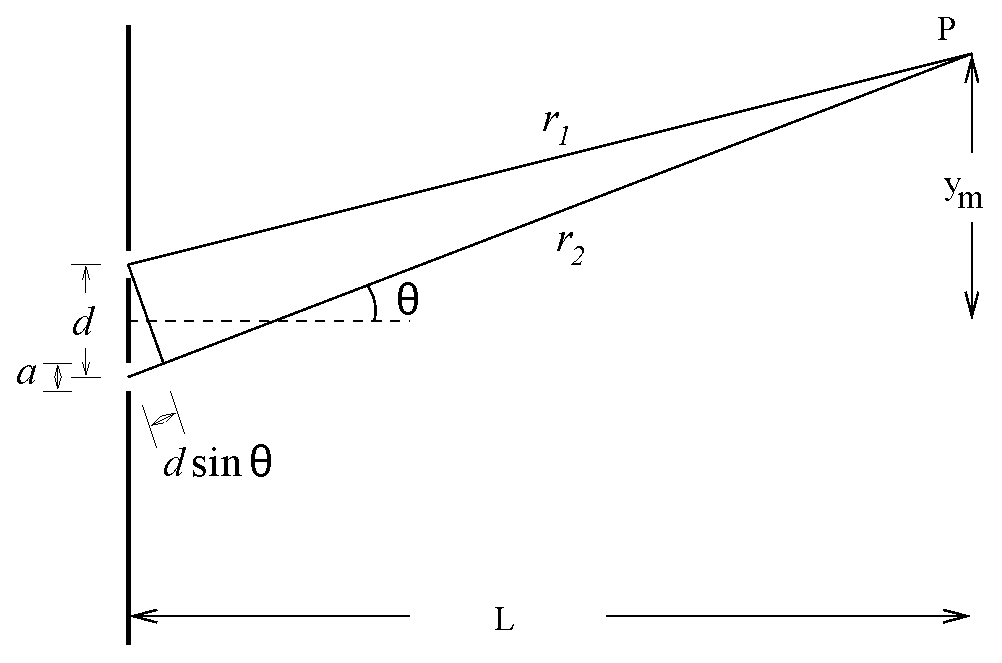
\includegraphics[scale=0.6]{10_diffraction/twoslit.eps}
\caption{The geometry of a simple two slit interference experiment.}
\label{fig:diff:2-slit}
\end{figure}

{\bf If the screen is far away from the slits}, $d \ll L$, then the two rays
between each slit and P are practically parallel. The phase difference arises
from the additional distance one ray must travel over the other. From the 
geometry of Fig.~\ref{fig:diff:2-slit}, we see that this distance is
$ \delta = r_2 - r_1 = d \sin \theta.$  If two waves have a path difference
that is an integer multiple of $\lambda$ ($\lambda, 2\lambda, \dots$) or
\begin{eqnarray}
\delta = d \sin \theta = m \lambda~~~{\rm (maxima)},
\label{eq:diff:2 slit maxima}
\end{eqnarray}
where $m$ is an integer (0,1,2,\dots), then they 
are in phase and constructive interference occurs.

For most (but not all) of the experiments we will do, the angles involved will be quite 
small.  The leading term in the Taylor series expansion of 
$\sin \theta$ is simply $\theta$; so if $\theta$ is small, the higher order 
terms are unimportant. So,
\begin{eqnarray*}
\sin \theta \sim \theta~~~{\rm (\mbox{for }\theta \ll 1)}.
\end{eqnarray*}
\begin{figure}[htb]
\centering 
\epsfxsize=4cm 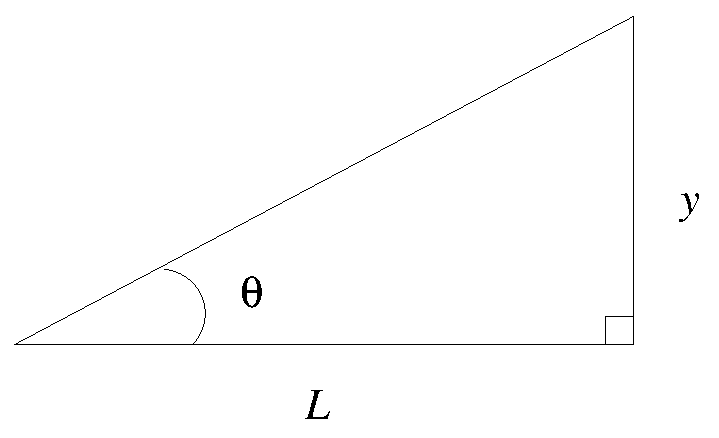
\includegraphics[scale=0.4]{10_diffraction/triangle.eps}
\caption{The triangle used to relate $\sin\theta$ to $y$ and $L$.} 
\label{fig:diff:triangle}
\end{figure}
Now, if we have a right triangle with $\theta$ as one of the acute angles, and
legs with lengths $y$ and $L$, $L \gg y$ (see Fig.~\ref{fig:diff:triangle}), 
then we can approximate
\begin{eqnarray*}
\sin \theta &\sim& \theta \\
\frac{y}{\sqrt{y^2+L^2}} &=& \frac{y}{L}
\frac{1}{\sqrt{1+\frac{y^2}{L^2}}}
\sim \frac{y}{L}
\end{eqnarray*}
so that we arrive at the {\em small angle approximation} $\theta \sim y/L$.
In the small angle approximation, Eq.~\ref{eq:diff:2 slit maxima}
becomes
\begin{eqnarray}
\fbox{$ \displaystyle y_m=m \lambda \frac{L}{d} $}~~~{\rm (maxima)}
\end{eqnarray}
where $y_m$ is the distance from the centerline to the $m$th maximum.
We can also predict where the minimum intensity should occur; simply set
the integer multiple of $\delta$ equal to $(2m+1) \frac{\lambda}{2}$,
i.e. odd multiples of half-wavelength.
We can gain some quick intuition about the behavior of this interference 
pattern by looking at the widths of the maxima; this quantity, $w$, 
we define as the distance between successive minima:
\begin{eqnarray*}
w = y_{m+1}-y_m \sim \lambda \frac{L}{d}
\end{eqnarray*}
which indicates that the {\it width grows as the distance between the slits 
decreases}. This is a common feature of interference and 
diffraction, as we shall see.

We now know the distance to the bright area but we also want to know
how the intensity varies with distance, which we will determine
graphically using phasors following Serway's example.

In the two-slit experiment, we have two sinusoidal waves with 
electric field components given by
\begin{equation}
E_1 = E_0 sin(\omega t) \mbox{ and }E_2 = E_0 sin(\omega t + \phi),
\label{eqn:diff:E1E2}
\end{equation}
where $E_0$ is the wave amplitude, $\omega$ is the wave angular frequency,
and $\phi$ is the phase difference.  Note that since we have one source of 
light illuminating both slits, $\omega$ is the same for both waves and $\phi=0$
at the slits. However, the phase difference is no longer zero at the
screen.  The phase difference at point P depends on the path difference,
$\delta = r_2 - r_1 = d\sin \theta$.  We want a relationship between phase
difference, $\phi$, and the angle $\theta$.  A path difference of $\lambda$
for constructive interference corresponds to a phase difference of $2\pi$
radians while a path difference of $\lambda /2$ for destructive interference 
corresponds to a phase difference of $\pi$ radians.  We obtain the ratio
\begin{eqnarray}
\frac{\delta}{\phi} &=& \frac{\lambda}{2 \pi} \nonumber \\
\phi &=& \frac{2 \pi}{\lambda} \delta = \frac{2 \pi}{\lambda} d \sin \theta. 
\label{eqn:diff:phase difference}
\end{eqnarray}

\begin{figure}[htb]
\centering 
\epsfxsize=4cm 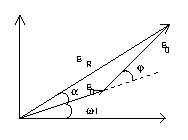
\includegraphics[scale=1.5]{10_diffraction/2E.eps}
\caption{Graphical representation of the resultant $E_R$.} 
\label{fig:diff:2E}
\end{figure}

The waves in Eq.~\ref{eqn:diff:E1E2} are represented graphically 
in Fig.~\ref{fig:diff:2E}.
We shall use the phasor method to graphically determine the intensity
of the pattern we will see on the screen; this is obtained by drawing the 
second vector at an angle $\phi$ with respect to the first.  
Let's review the phasor addition
of two waves such as $E_1$ and $E_2$.  The resultant wave, $E_R$ is the
sum of the two waves as
given in Fig.~\ref{fig:diff:2E}.  From the geometry of Fig.~\ref{fig:diff:2E}
one can find
\begin{eqnarray}
E_R & = & E_0 \cos \alpha + E_0  \cos \alpha  = 2 E_0 \cos \alpha \\
   & = & 2E_0 \cos (\phi/2)
\end{eqnarray} 
The projection of $E_R$ on the vertical 
axis is $E_P$,
\begin{eqnarray}
E_P & = & E_R \sin (\omega t + \alpha) = E_R \sin (\omega t + \phi/2) \\
    & = & 2 E_0 \cos( \phi/2) \sin (\omega t + \phi/2).
\end{eqnarray}
Knowing that the intensity of the light is $I=c \epsilon_0 E_P^2$, one can find
\begin{equation}
I = 4 c \epsilon_0 E_0^2 \cos^2(\phi/2)\sin^2(\omega t + \phi/2);
\end{equation}
however, most light detecting instruments detect the time-average intensity 
of light.
The time average of $\sin ^2 (\omega t + \phi/2)$ is $1/2$ so the average 
intensity at P is
$$
I_{avg} = I_0 \cos ^2 (\phi/2) 
$$
where $I_0$ is the maximum possible time average light intensity and
$I_0 = 2 c \epsilon_0 E_0^2$.
Using Eq.~\ref{eqn:diff:phase difference} 
into the above equation for $I_{avg}$,
\begin{equation}
\fbox{$ \displaystyle I_{avg} = I_0 \cos^2 (\frac{\pi d \sin \theta}{\lambda})$}
\label{eqn:diff:Iavg}
\end{equation}
Indeed, the function~\ref{eqn:diff:Iavg} is a simple $\sim \cos^2 \alpha$
function, which has the simple structure as seen in the top part ($n=2$) of 
Fig.~\ref{fig:diff:intnodiff} below. 

For our specific example of two-slit interference,
Fig.~\ref{fig:diff:phasors_2slit} represents the phasor 
diagrams for various values of $\phi$ (and therefore $\delta$).  
Noting that $I$ will be at a maximum when $E_R$ is at a maximum,
we see that the intensity is at a maximum at $\phi = 0,2\pi,\dots$ and 
$I = 0$ when $E_R=0$ at $\phi = \pi,3\pi,\dots $.
\pagebreak  
\begin{figure}[htb]
\centering 
\epsfxsize=12cm 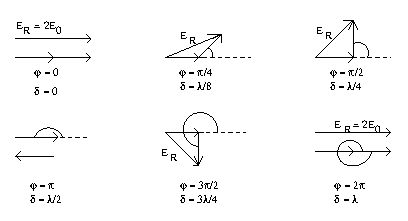
\includegraphics[scale=2.0]{10_diffraction/phasors_2slit.eps}
\caption{The phasor diagram for two-slits.}
\label{fig:diff:phasors_2slit}
\end{figure}
 
\subsection{Multiple-Slit Interference}
Now we consider what happens when we have more than two slits.
We will determine a general formula for $n$ slits, but let's first
do the three-slit problem in some detail.  Following the two-slit
analysis, we once again use phasors to determine the intensity
of the light that will be reaching the screen. 
Now we have three waves (see Fig.~\ref{fig:diff:3E}), namely
\begin{eqnarray}
E_1 & = & E_0 \sin( \omega t) \\
E_2 & = & E_0 \sin( \omega t+ \phi) \\
E_3 & = & E_0 \sin( \omega t + 2 \phi). 
\end{eqnarray}
\pagebreak
\begin{figure}[htb]
\centering 
\epsfxsize=4cm 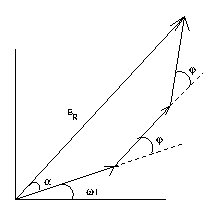
\includegraphics[scale=1.4]{10_diffraction/3E.eps}
\caption{Resultant of three waves.}
\label{fig:diff:3E}
\end{figure}

The phasor diagrams for various values of $\phi$ for the three-slit experiment
is given in Fig.~\ref{fig:diff:phasors_3slit}.
\begin{figure}[htb]
\centering 
\epsfxsize=14cm 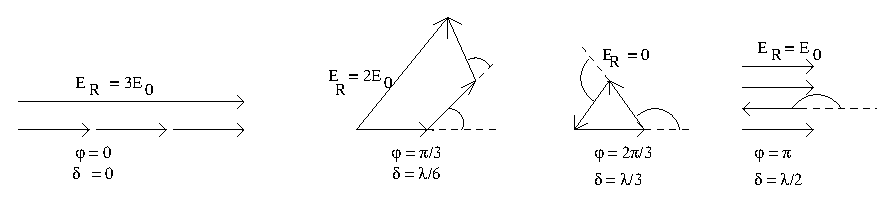
\includegraphics{10_diffraction/phasors_3slit.eps}
\caption{Phasor Diagram for Three Slits.}
\label{fig:diff:phasors_3slit}
\end{figure}
These diagrams tell us that there are both primary maxima 
and secondary maxima.  The primary maxima have resultant values, $E_R = 3E_0$
when $\phi = 0, \pm2 \pi, \pm 4 \pi,\dots$.  This is the case when the three 
phasors are aligned.  The secondary maxima have $E_R = E_0$ when 
$\phi = \pm \pi, \pm 3\pi,\dots$.  This pattern is shown as the second plot 
($n=3$) of Fig.~\ref{fig:diff:intnodiff}.  At these points, one of the waves
exactly cancels another leaving a third.  Notice that the two-slit
pattern did not have any secondary maxima while the three-slit pattern had
one secondary maxima.  The intensity can be found from the projection
of the resultant electric field, $E_R$, as in the two-slit case.  The
result is
\begin{equation}
I   =  I_0 \frac{\sin^2 \left(m \pi \frac{d}{\lambda} \sin \theta\right)}
                 {\sin^2 \left(  \pi \frac{d}{\lambda} \sin \theta\right)}
\label{eqn:diff:multiI}
\end{equation}
where $I_0 = \epsilon_0 E_P^2/2$. One can show that, when $n=2$,
this takes the form (Hint: use $\sin 2x = 2 \sin x \cos x$)
$$I=4I_0\cos^2\left(\pi \frac{d}{\lambda} \sin \theta\right).$$
Figure~\ref{fig:diff:intnodiff} schematically represents
the intensity pattern for 2, 3, 4, and 5 slits.
You can see that the number of secondary maxima increase with increasing 
slit number, $n$.

\begin{figure}[htb]
\centering 
\epsfxsize=6cm 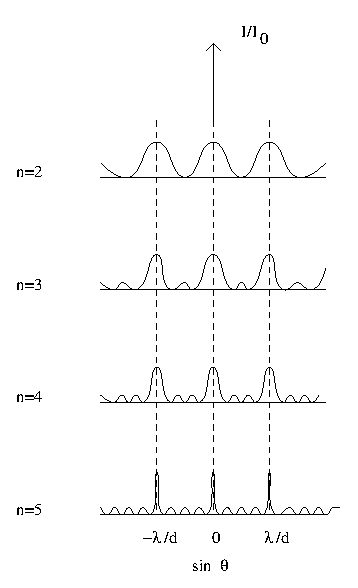
\includegraphics{10_diffraction/internodiff.eps}
\caption{Interference pattern for 2, 3, 4, and 5 slits without diffraction.}
\label{fig:diff:intnodiff}
\end{figure}

\subsection{Diffraction Grating}

We can use our multiple-slit pattern to examine a very useful device:
the diffraction grating. This is a plate that has thousands of slits cut into 
it.  Gratings with many lines per cm have a very small slit spacing, $d = 
1/(\mathrm{lines}/\mathrm{cm})$.  A piece of the grating is illustrated in 
Fig.~\ref{fig:diff:grating}.
\begin{figure}[htb]
\centering 
\epsfxsize=6cm 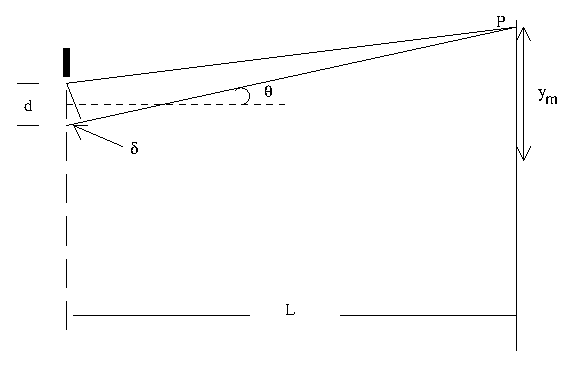
\includegraphics{10_diffraction/grating.eps}
\caption{Set-up for diffraction grating.}
\label{fig:diff:grating}
\end{figure} 
Each slit acts like a source of waves; therefore, each slit produces a
wave which interferes with the other waves from the other slits.  As in the
two-slit case, each wave is in phase at the grating, but travels,
relative to its immediate neighbor, a different
path length to the point P on the screen, $\delta = d \sin \theta$.  
When the path length difference equals a multiple of the wavelength, all the waves
are in phase and a bright spot appears on the screen; therefore, the 
condition for maxima in the interference pattern at angle $\theta$ is 
\begin{eqnarray}
\fbox{$ \displaystyle d \sin \theta = m \lambda $},
\end{eqnarray}
for some integer $m$ where  
$m$ is called the {\em order} of the fringe. Knowing the slit spacing~$d$, the 
order of the fringe and measuring $\sin \theta$ will produce a fairly precise
measurement of the wavelength.  The intensity of the diffraction grating versus
the angle, $\theta$, is shown in Fig.~\ref{fig:diff:diffgratI}.  Note
the sharply peaked bright areas and the wider dark areas,  we will be seeing
this in the diffraction grating experiment.
\begin{figure}[htb]
\centering 
\epsfxsize=6cm 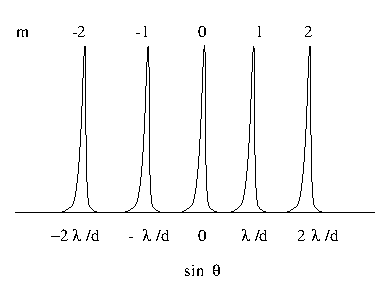
\includegraphics[scale=1.0]{10_diffraction/diffractI.eps}
\caption{Intensity pattern for diffraction grating}
\label{fig:diff:diffgratI}
\end{figure}

\subsection{Single-Slit Diffraction and Available Light}
\label{sec:diff:singleslit}

We have been assuming that the slit is so much smaller then the wavelength,
$a \ll \lambda$ that each slit acts like a point source of light.  However,
in the experiments today our slits are on the order of a wavelength, 
$a \sim \lambda$ so we need to take diffraction into consideration.
We will see (Fig.~\ref{fig:diff:multislit diffraction}) that diffraction
has the effect of diminishing the available light for the interference pattern
to be seen.

We can observe the effect of diminishing light when we place a 
single slit in front of the laser beam.  We will find a surprising
result: the beam gets distorted and fringes appear in 
the shadow zone of the slit.
To describe this phenomenon, known as diffraction, we can use Huygen's 
principle. According to this idea, we can treat the single slit as a bunch of
really, really small single slits and let them interfere with one another. So,
let our real slit have a width $a$ and consider a small subset of this region
with a width $\Delta y$ located a distance $y$ from the center, as shown in 
Fig.~\ref{fig:diff:single slit diffraction}.
\begin{figure}[htb]
\centering 
\epsfxsize=8cm 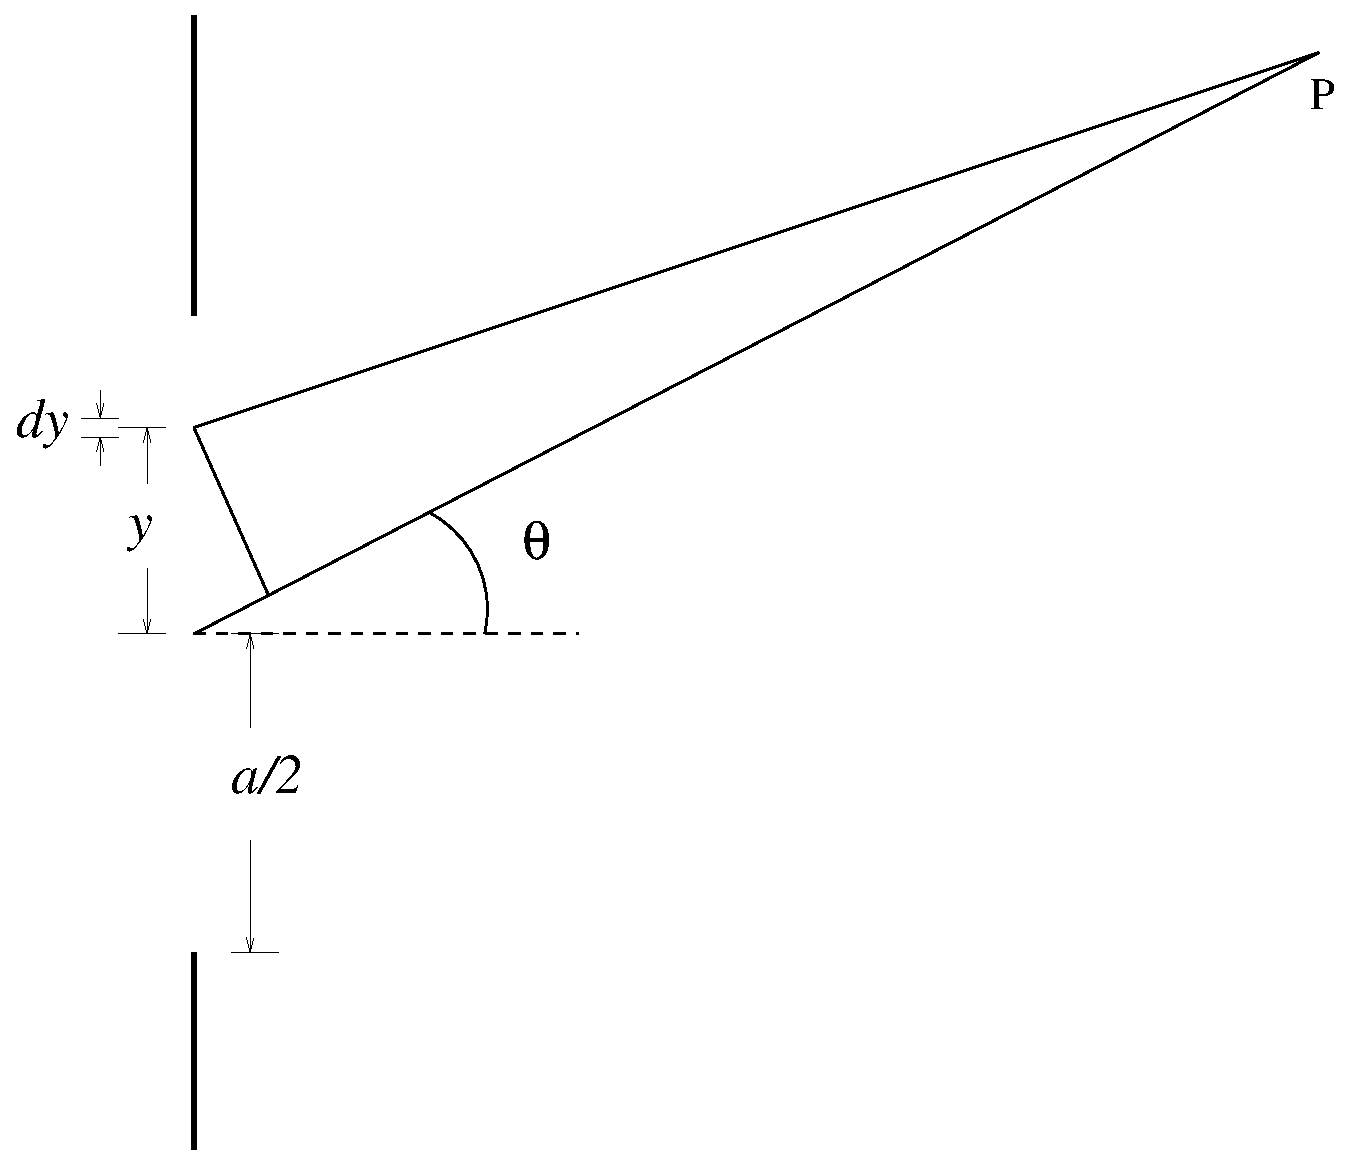
\includegraphics[scale=0.6]{10_diffraction/singlediff.eps}
\caption{Configuration for analyzing single slit diffraction using Huygen's
principle.}
\label{fig:diff:single slit diffraction}
\end{figure}
Now, the phase difference between a ray at  our miniture slit at $y$ and one at
the center is $\phi(y)  = m y \sin \theta$, where we have again 
assumed that the rays leaving are practically parallel and that 
$m$ is an integer.
By using phasors where each portion of the slit contributes an electric
field amplitude, $E$, one can once again solve for the 
intensity of the resulting
diffraction pattern as seen on the screen at some point P.  We will not go
through this procedure since it follows the n-slit procedure.
The resulting intensity is
\begin{equation}
I_{\theta} = I_0 \left [ \frac{\sin (\pi a \sin \theta / \lambda )}
{\pi a \sin \theta / \lambda}\right] ^2,
\label{eqn:diff:singleI}
\end{equation}  
which is plotted in Fig.~\ref{fig:diff:singlediffI} as a function of 
$\theta$ for $a = 3 \lambda$.  This pattern depicts
the intensity of light available at various points from a single slit.
\begin{figure}[htb]
\centering 
\epsfxsize=8cm \includegraphics[scale=0.6]{10_diffraction/singslitpatt.eps}
\caption{Intensity pattern for a single slit diffraction experiment.}
\label{fig:diff:singlediffI}
\end{figure}

The position of the {\bf minima} are at angles given by
\begin{eqnarray*}
\sin \theta = \frac{m \lambda}{a}~~~{\rm (minima)}
\end{eqnarray*}
which is the same as the two-slit interference {\bf maxima} with the slit 
separation
$d$ replaced by the slit width $a$.
The $m=1$ minima position ($\sin \theta = \frac{\lambda}{a}$) shows that the 
pattern expands as the slit width decreases.  When $a < \lambda$, minima no
longer occur and the pattern begins to resemble the point source pattern at the
bottom of Fig.~\ref{fig:diff:opening}.
\suppressfloats

\subsection{Multiple-Slit Diffraction}
\label{sec:diff:multislit}

You can go through a similar calculation for multiple-slit diffraction 
patterns; but, we can also be a bit smarter about it and save ourselves some 
work. Notice that the diffraction of a single slit will not affect the 
treatment of interference of multiple slits because you simply add the 
corresponding contributions from the various slits with the appropriate phase
factors. Because the single-slit diffraction pattern determines whether
the light will be available for interference at a given point, 
the result simply
becomes the product of the single-slit diffraction pattern 
(Eq.~\ref{eqn:diff:singleI}) and the multiple-slit 
interference pattern (Eq.~\ref{eqn:diff:multiI}). 
\begin{eqnarray}
I = I_0 \frac{\sin^2 \left(\frac{n\pi d}{\lambda} \sin \theta \right)}{
\sin^2 \left(\frac{\pi d}{\lambda} \sin \theta\right)}
        \frac{\sin^2 \left( \frac{\pi a}{\lambda} \sin \theta\right)}{
        \left( \frac{\pi a}{\lambda} \sin \theta  \right)^2}
    \label{eq:diff:multislit diffraction intensity}
\end{eqnarray}
This is what you will observe in the lab. We provide a graph of this intensity 
in Fig.~\ref{fig:diff:multislit diffraction} for $n=2$.
\begin{figure}
\centering 
\epsfysize=8cm \includegraphics[scale=0.6]{10_diffraction/envelope.eps}
\caption{Multiple-slit diffraction pattern for $n=2$.}
\label{fig:diff:multislit diffraction}
\end{figure}
Since $a < d$ (the slits do no overlap), 
the diffraction minima occur farther apart than the 
interference minima; this means that the diffraction pattern really forms an 
envelope for the interference patterns (see Fig.~\ref{fig:diff:intpatt}).
\newpage
\begin{figure}
\centering 
\epsfysize=12.5cm 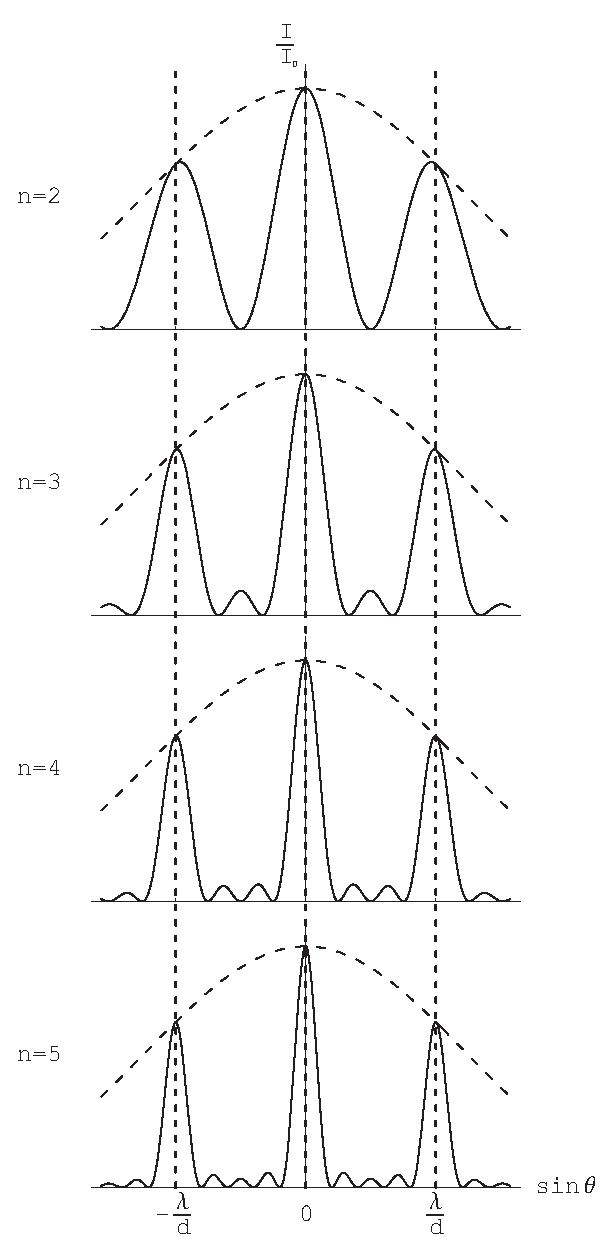
\includegraphics[scale=0.6]{10_diffraction/interferencepatt.eps}
\caption{Interference pattern for 2, 3, 4, and 5 slits with diffraction}
\label{fig:diff:intpatt}
\end{figure}

\section{Apparatus}

The apparatus for this lab is rather simple.  We'll use the lasers as light 
sources, since we need a monochromatic beam of light to clearly illustrate the
effects of interference and diffraction. Please recall the guidelines for 
laser safety given in Lab~\ref{ch:optics}. We'll use an adjustable single
slit to study single slit diffraction, a slide with multiple-slit patterns, and
a diffraction grating slide.

\vfill
\pagebreak
$$
$$
\vfill
\clearpage
\newpage


%  Label worksheets by \thechapter.W
\renewcommand{\thesection}{\thechapter.W}

\section{Diffraction and Interference Worksheet}
{\bf \Large Name:}~ \rule{5cm}{.1mm}~~~~~~~
{\bf \Large Day/Time:}~\rule{3cm}{.1mm}\\ 
{\bf \large Partners' Names:}~\rule{6cm}{.1mm}\\

\subsection{In-Lab Procedure}

For most of the procedures in this lab, we will require a distance of at least
2~m between the slit assembly and the screen you'll use to observe the pattern;
$L$ must be large for the small angle approximation.  As a screen, we'll 
use large sheets of computer paper taped to the wall; these are nice, because 
you can easily trace the pattern on them.  However, this means that several 
groups of students will have to aim the lasers {\it across} the room.  As long
as everyone is careful not to aim their own lasers up at eye level and we 
remain aware of everyone else's lasers, there should be no problems.  Be 
patient and understanding if your instructor or a classmate needs to walk in
front of your beam when you're in the middle of making a sketch.
 
\subsubsection{Single-Slit Diffraction}  

Find a convenient way to aim the laser at one of the walls so that there's
no electrical outlet or other obstruction to taping your paper screen onto the
wall; make sure that you will have at least a 2~m separation between the 
{\it slit assembly} and the wall.  Place the single-slit apparatus in front of 
the laser and align the slit with the beam. This may take a bit of playing 
around; try placing the slit apparatus on its side or prop it up if necessary. 
You might also need to adjust the slit width; just be careful not to look 
directly into the laser beam or its reflections.  When you have the slit set 
up properly, you should see a pattern of {\it spots}. \\ 
\vspace*{.3cm} \\
{\bf Question 0}: What does this pattern, 
specifically the brightness of the spots, have to do with 
Fig.~\ref{fig:diff:singlediffI}?   \\
\clearpage

\noindent Trace {\bf two} patterns: one with a relatively large slit 
width and another with a 
relatively small slit width; make sure that you label these appropriately.   
You will use these traces to answer a series of questions in the In-Classroom
Calculation \& Analysis section.  


\subsubsection{Multiple-Slit Diffraction/Interference Patterns} 
\label{sec:diff:multislitproc}

\noindent Replace the single slit assembly with the multiple-slit slide
(mounted in a magnetic holder). Using a length of string and a meter-stick, 
measure the distance from the slide to the screen, $L$, and record this value
below with uncertainty.
\begin{center}
$L=$~ \rule{3cm}{.1mm} 
\end{center}
Adjust the slide
so that the two slit pattern (slit pattern, not interference pattern) is 
directly in front of the beam; adjust it until you get a clear interference 
pattern on the screen. Record the slit spacing $d$ below.

\begin{center}
$d=$~ \rule{3cm}{.1mm}
\end{center}
\vspace*{.5cm}

\begin{figure}[htb]
\centering 
\epsfxsize=15cm 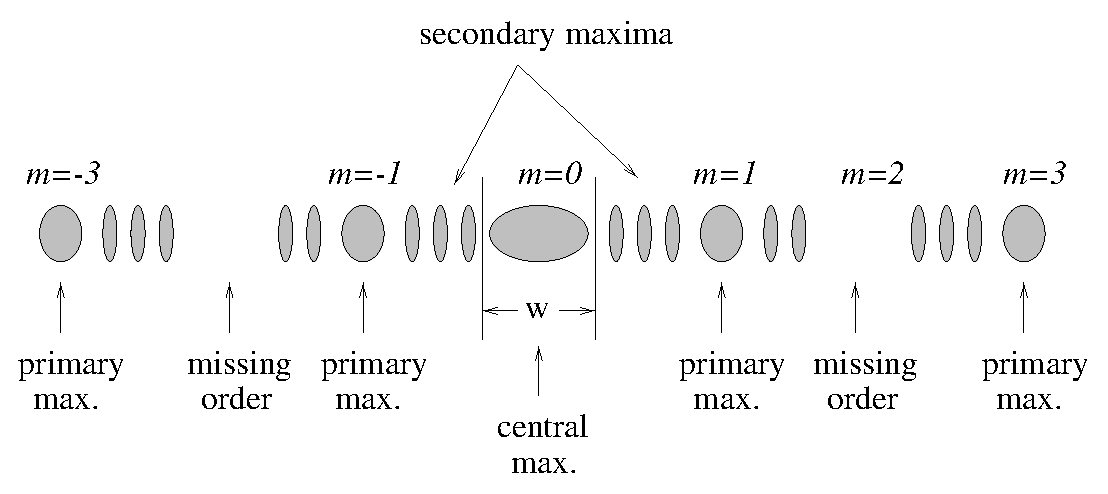
\includegraphics[scale=0.6]{10_diffraction/interpatt.eps}
\caption{The interference/diffraction pattern for 5 slits.}
\label{fig:diff:interpatt}
\end{figure}

\noindent Trace the {\bf two} slit pattern (remember to label it). 
When doing the trace,
make sure you are able to trace at least {\bf eight primary} maxima. (Four
primary maxima on each side of the central maximum is preferable).
Determine the orders of each of the primary maxima on your trace of
the two-slit interference pattern. Refer to Fig.~\ref{fig:diff:interpatt}
for guidance but note that this figure is of a 5-slit pattern.
Measure the distances $y_m$ for at least 8 primary maxima; remember to skip
the missing orders when you do this; once again 
referring  to Fig.~\ref{fig:diff:interpatt} for guidance. \\

\noindent
Measure the distances $y_m$ from the $m$th primary maximum to the
center of the central maximum for at least eight primary maxima. {\bf
Note: The values of $y_m$ for negative $m$ should be taken to be
negative}. Record your eight $y_m$ vs. $m$ measurements into 
Table~\ref{tab:DI:twoslit}.

\begin{table}[htb]
\begin{center}
\begin{tabular}{|c|c|c|c|c|}
\hline
\multicolumn{5}{|c|}{Measurements of $y_m$ vs. $m$ for Two-slit Diffraction Pattern.} \\
\hline
Distance ($y_m$) & Order ($m$) & & Distance ($y_m$) & Order ($m$) \\
\hline
\hspace*{3cm} & \hspace*{3cm} & \hspace*{.3cm} & \hspace*{3cm} & \hspace*{3cm} \\
& & & & \\
\hline
& & & & \\ & & & & \\
\hline
& & & & \\ & & & & \\
\hline
& & & & \\ & & & & \\
\hline
\end{tabular}
\end{center}
\caption{$y_m$ vs. $m$ measurements for two-slit diffraction pattern.}
\label {tab:DI:twoslit}
\end{table}

\ \\
\noindent 
Let's also examine the qualitative properties of the other slit
patterns.  Observe the patterns for the 3, 4, and 5 slit patterns; you
don't need to sketch them.  Is there anything discussed in
Section~\ref{sec:diff:multislit} that you can compare this behavior
with?  Record below the results of your observations of the {\it
qualitative} properties of the interference patterns resulting from 3,
4, and 5 slits. In particular, answer the following two questions. 
\vspace*{.5cm}

\noindent 
{\bf Question 1}: For each of the 3, 4, and 5 slit patterns, how many
secondary maxima appear between primary maxima?
\vspace*{.8cm}

\noindent
{\bf Question 2}: What happens to the size of the primary maxima as you
increase the number of slits?\\








\subsubsection{Diffraction Grating Pattern} 

Replace the multiple-slit slide with the diffraction grating slide.  Can you
see the diffraction pattern?  What if you place a sheet of paper directly in
front of the grating? Adjust the grating-to-screen distance until you can see
five dots, as illustrated in Fig.~\ref{fig:diff:diffgratpat}. 
\begin{figure}[htb]
\centering 
\epsfxsize=8cm 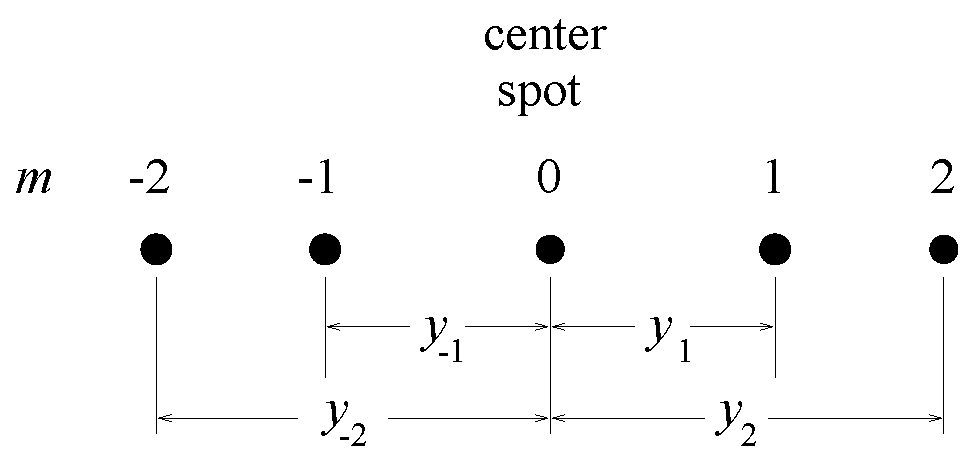
\includegraphics[scale=0.6]{10_diffraction/diffpatt.eps}
\caption{The interference pattern from the diffraction grating.} 
\label{fig:diff:diffgratpat}
\end{figure}

\noindent
Measure the grating-to-screen distance, $L_g$, and write down the number of 
lines/cm, $s,$
as printed on the grating slide. 

\begin{center}
$L_g=$~ \rule{3cm}{.1mm} ~~~~ $s=$~ \rule{3cm}{.1mm}
\end{center}
\vspace*{.5cm}
\noindent  Now trace the 5~bright spots that form the 
interference pattern. Some dim spots may appear above and/or below the bright 
ones; these are due to imperfections in the grating and we may ignore them. \\

\noindent 
On your trace of the diffraction grating interference pattern, assign
a value $m$ to each of the dots. Refer to Fig.~\ref{fig:diff:diffgratpat}
to see how.  Measure the distances $y_m$ from the $m$th dot to the center 
dot for
all five of the dots. {\bf Note:} Again, the values of $y_m$ for
negative $m$ should be taken to be negative, see 
Fig.~\ref{fig:diff:gratgraph}. 


\begin{figure}[htb]
\centering 
\epsfxsize=7cm 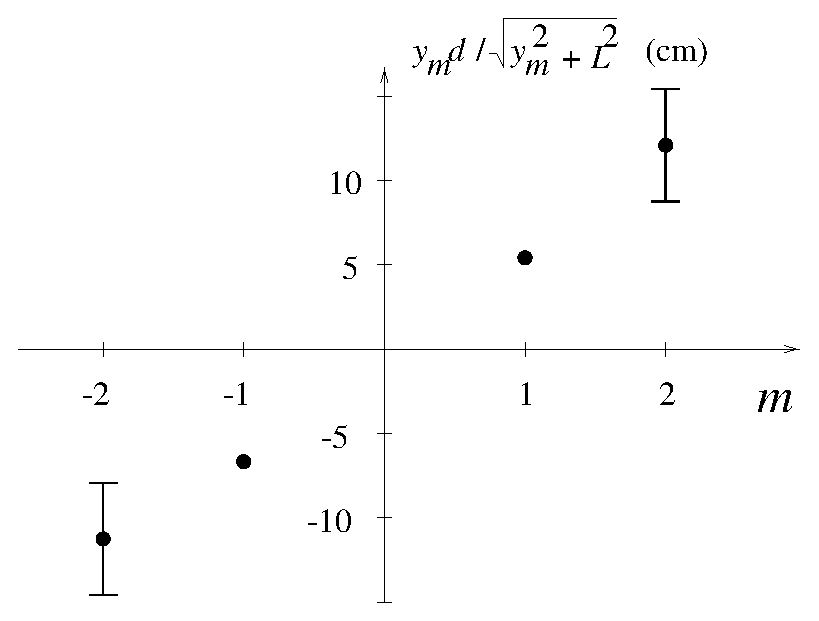
\includegraphics[scale=0.6]{10_diffraction/gratgraph.eps}
\caption{An illustration of a typical graph of the grating data.}
\label{fig:diff:gratgraph}
\end{figure}
\vspace*{1cm} 
\noindent 
Record your five $y_m$
vs. $m$ measurements into Table~\ref{tab:DI:Grating}.
\begin{table}[htb]
\begin{center}
\begin{tabular}{|c|c|}
\hline
\multicolumn{2}{|c|}{Measurements of $y_m$ vs. $m$} \\
\hline
Distance ($y_m$) & Order ($m$) \\
\hline
\hspace*{3cm} & \hspace*{3cm}  \\
& \\
\hline
& \\ & \\
\hline
& \\ & \\
\hline
& \\ & \\
\hline
& \\ & \\
\hline
\end{tabular}
\end{center}
\caption{$y_m$ vs. $m$ measurements for diffraction grating pattern.}
\label {tab:DI:Grating}
\end{table}
 
\clearpage

\subsection{In-Lab Computer Work}


\subsubsection{Multiple-Slit Diffraction/Interference Patterns}

Using the measured values in Table~\ref{tab:DI:twoslit}, calculate
$y_md/L$ and its uncertainty for one set of data.  
{\bf Show all work} in the space provided
below. \\
\vspace*{4cm} \\
\noindent Make a plot (with error bars) of $y_md/L$ vs. $m$ 
Find the slope of the weighted best fit line, and record this
below with uncertainty.

\begin{center}
$S_1$=~ \rule{3cm}{.1mm}
\end{center}


\subsubsection{Diffraction Grating Pattern}

Using the measured values in Table~\ref{tab:DI:Grating}, calculate
$y_md/ \sqrt{y_m^2 + L_g^2}$ and its uncertainty for one set of data.  
{\bf Show all work} in the space provided below. \\
\vspace*{5cm} \\

\noindent Now, plot $y_md/ \sqrt{y_m^2 + L_g^2}$ vs. $m$ with error bars. 
Find the
slope of the weighted best fit line, and record this below with
uncertainty.

\begin{center}
$S_2$=~ \rule{3cm}{.1mm}
\end{center}

\subsection{Pre-Classroom Check List}
$\bigcirc$ \hspace*{1cm} One partner has two labeled tracings from single slit \\
$\bigcirc$ \hspace*{1cm} One partner has a labeled tracing from two slit \\
$\bigcirc$ \hspace*{1cm} One partner has a labeled tracing from grating \\
$\bigcirc$ \hspace*{1cm} Table~\ref{tab:DI:twoslit} completed with units and uncertainties \\
$\bigcirc$ \hspace*{1cm} Table~\ref{tab:DI:Grating} completed with units and uncertainties \\
$\bigcirc$ \hspace*{1cm} $S_1$ with uncertainty and units \\
$\bigcirc$ \hspace*{1cm} $S_2$ with uncertainty and units \\
$\bigcirc$ \hspace*{1cm} 2 Plots labeled completely and correctly \\
$\bigcirc$ \hspace*{1cm} Each student has her/his own plots and worksheet \\
 


\subsection{In-Classroom Calculations \& Analysis}


From your value for $S_1$, determine the value of the wavelength of
the laser light for your two-slit interference pattern, $\lambda _1,$
with uncertainty. \\
\vspace*{2cm} \\
\begin{center}
$\lambda _1=$~ \rule{3cm}{.1mm} 
\end{center}
\noindent From your value of $S_2$, determine the value of
the wavelength of the laser light for your diffraction grating
interference pattern, $\lambda _2$ with uncertainty. \\
\vspace*{2cm} \\
\begin{center}
$\lambda _2=$~ \rule{3cm}{.1mm}
\end{center}

\noindent
From $\lambda _1$ and $\lambda _2$ calculate the average wavelength
with standard deviation. {\bf Note:} Use Eq.~(0.1) and Eq.~(0.2) in
$\S$~\ref{sec:intro:uncert}. Record the average value $\lambda
_{avg}$ below with uncertainty. \\
\vspace*{3cm} \\ 
\begin{center}
$\lambda _{avg}=$~ \rule{3cm}{.1mm}
\end{center}

\subsection{In-Classroom Discussion}
\subsubsection{Single-Slit Diffraction}
Refer to the traces you made of the single-slit diffraction patterns.
Is the small angle approximation valid for analyzing these traces?
Explain.
\vspace*{2cm}

\noindent 
What happened to the width of the spots in the single-slit diffraction
pattern as you increased the slit width?
\vspace*{2cm}

\noindent
What happened to the separation between the spots in the single-slit
diffraction pattern as you increased the slit width?
\vspace*{2cm}

\noindent
Do your answers to the above two questions agree qualitatively with
the results obtained in 
$\S$~\ref{sec:diff:singleslit}? Explain by citing the relevant results. \\
\vspace*{2cm} \\

\subsubsection{Multiple Slit Diffraction/Interference Patterns}
What is responsible for the existence of missing orders in a multiple
slit interference pattern? (Hint: examine 
Fig.~\ref{fig:diff:multislit diffraction}).  
\vspace*{1.4cm} 

\noindent
Is the small-angle approximation valid for analyzing your trace of the
two-slit interference pattern? Explain by comparing your largest
$y_m$ value to $L.$
\vspace*{3cm}

\noindent
Is your plot of $y_md/L$ vs. $m$ linear within error?
\vspace*{.3cm}

\noindent
Compare your value of $\lambda _1$ to the known wavelength of He-Ne
light, 632.8 nm.
\vspace*{2.5cm} 

\noindent
Does your observation of how the sizes of the primary maxima behave as
you increase the number of slits agree or disagree with the discussion
in $\S$~\ref{sec:diff:multislit}? Explain.
\vspace*{3cm}
  

\noindent
Referring to your trace of the two-slit interference pattern and the
qualitative observations you made about the 3, 4, and 5 slit
interference patterns, write an equation that relates the number of
slits, $n$, to the number of secondary maxima, $M,$ that occur in the
corresponding interference pattern. \\
\vspace*{2cm}


\subsubsection{Diffraction Grating Pattern}
Is your plot of $y_md/ \sqrt{y_m^2 + L_g^2}$ linear within error?
\vspace*{.3cm}

\noindent
Compare your value of $\lambda _2$ to the known wavelength of He-Ne
light, 632.8 nm.
\vspace*{1.4 cm}

\newpage


\noindent
Compare your value for $\lambda _{avg}$ with the known wavelength.
\vspace*{2.4cm}

\noindent
Which of the two methods of measuring wavelength is the most {\it
accurate}?
\vspace*{2cm}

\noindent
Is this expected? Why?
\vspace*{1cm}

\noindent
Do you gain anything by having made two separate measurements? What?
\vspace*{1.4cm} 

\newpage
\subsection{In-Classroom Conclusion}

Write a {\it brief} (that is, a one or two paragraph) conclusion for
this lab. In it, you should summarize the physical
principles which were meant to be illustrated in this experiment. You
should also describe the degree to which your data supported these
principles.


\vfill
\noindent Attach plots and tracings to the worksheet. \\
\ \\
{\Large End Worksheet} 

% Go back to ordinary section numbering
\renewcommand{\thesection}{\thechapter.\arabic{section}}

